\section{Datenanalyse}

	Dieser Abschnitt umfasst die Auswertung der aufgenommenen Daten.

\subsection{Verzögerungsdauer}
	
	Um möglichst viele Koinzidenzen zu messen, wird die Zählrate nach der Koinzidenzeinheit gegen die eingestellte Verzögerung aufgezeichnet.
	Hierzu wird $^{22}\text{Na}$ verwendet, um durch den Zerfall des Parapositroniums zwei $\gamma$-Quanten im Winkel von \SI{180}{\degree} zu gewährleisten.
	Die Überlagerungswahrscheinlichkeit ist durch eine Gauß-Kurve abgeschätzt und in \cref{fig:zeitdiff} dargestellt.
	\begin{figure}[ht]
		\centering
		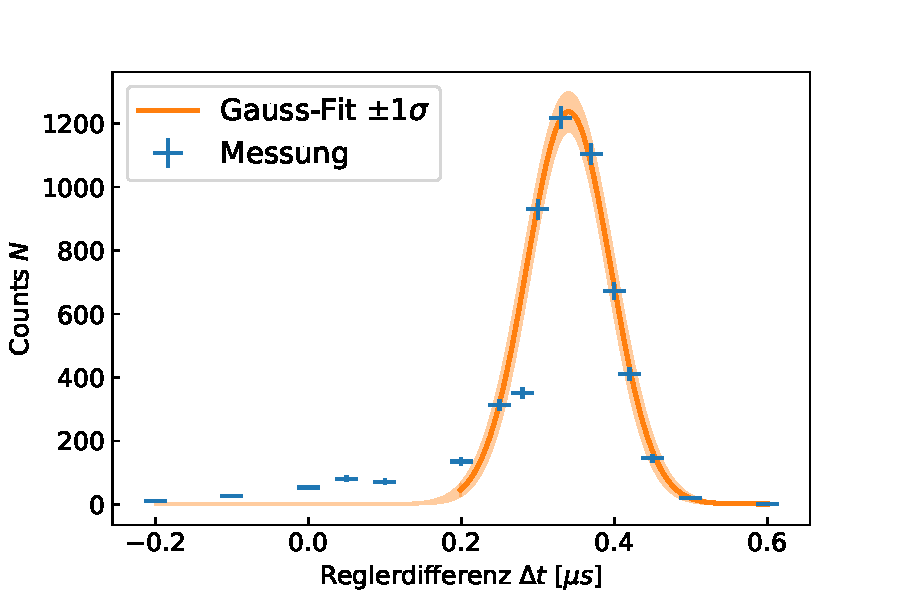
\includegraphics[width=0.7\textwidth]{dat/zeitdifferenz.pdf}
		\caption{Zusammenhang von der eingestellten Verzögerung zwischen beiden Signalen und der Zählrate.
			Die Daten wurden mit einer Gauß-Kurve $A \cdot \exp{-\frac{(\Delta t - \Delta t_0)^2}{2 \sigma_{\Delta t}^2}} + y_0$ angepasst.
			Alle konkreten Fit-Parameter finden sich in \cref{sec:fitval}.}
		\label{fig:zeitdiff}
	\end{figure}
	Da Werte mit Verzögerungsdauern kleiner als \SI{0.2}{\micro\second} eine statistisch relevante Abweichung von Null haben, wurden diese nicht in die Anpassung der Gauß-Kurve eingebunden.
	Die Position des Peaks liegt bei $\Delta t_0 = \input{dat/messung1_x0.txt}$.
	In allen folgenden Messungen ist die Signalverzögerung fest auf \SI{333}{\nano\second} eingestellt.
	Diese Einstellung ist mit der Peakposition kompatibel und liefert eine Signaleffizienz von $\epsilon = \input{dat/messung1_eff.txt}$ im Bezug zum Peakmaximum.
	Die Breite $\sigma_{\Delta t} = \input{dat/messung1_d.txt}$ der Kurve ist eine grobe Abschätzung für die Zeitauflösung.
	
\subsection{Koinzidenzauflösungszeit}
	
	Eine genauere Bestimmung der Auflösungszeit $2\theta$ von zwei aufeinander folgenden Signalen ist mit
	\begin{equation}
		N_Z = N_1 \cdot N_2 \cdot 2\tau \Leftrightarrow 2\tau = \frac{N_Z}{N_1 N_2} = \input{dat/messung2_zweiT.txt}
	\end{equation}
	möglich.
	Dabei sind $N_1 = \input{dat/messung2_det1.txt}$, $N_2 = \input{dat/messung2_det2.txt}$ die Zählraten beider Detektoren vor und $N_Z = \input{dat/messung2_koinz.txt}$ die Zählrate nach der Koinzidenzeinheit.
	Die Probe hatte im Jahr 1962 eine Aktivität von \SI{3.7}{\mega\becquerel} und somit werden bei der Messung ca. \SI{0.4}{\%} aller Zerfälle gemessen.
	Das errechnete Ergebnis liegt in der Größenordnung der Abschätzung.
		
\subsection{Vernichtungsstrahung}

	\begin{figure}[ht]
		\centering
		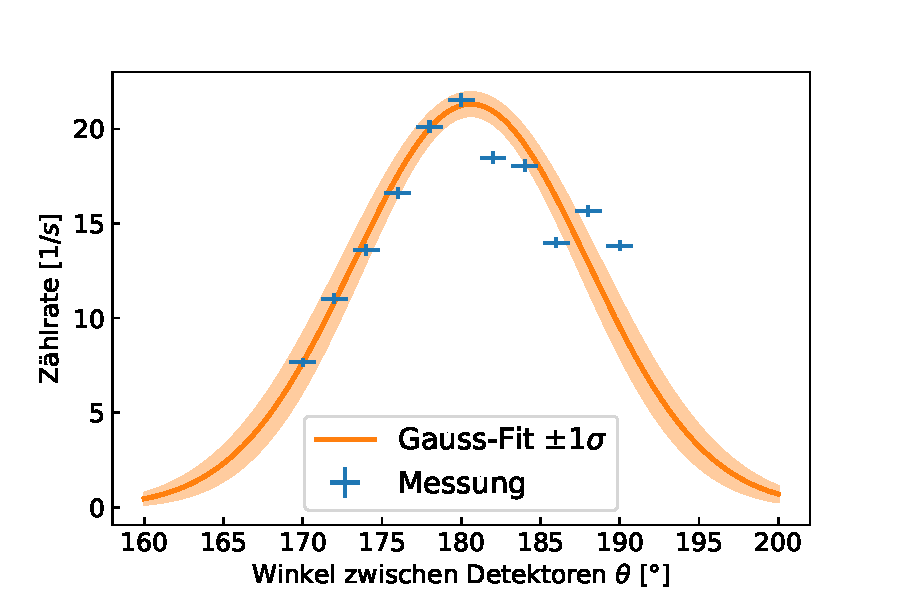
\includegraphics[width=0.7\textwidth]{dat/vernichtung.pdf}
		\caption{Winkelauflösung der Detektoren.}
		\label{fig:vernichtung}
	\end{figure}
	%TODO mit 0,4% aus sec2 übereinstimmend?

\subsection{Winkelkorrelation}

	\begin{figure}[ht]
		\centering
		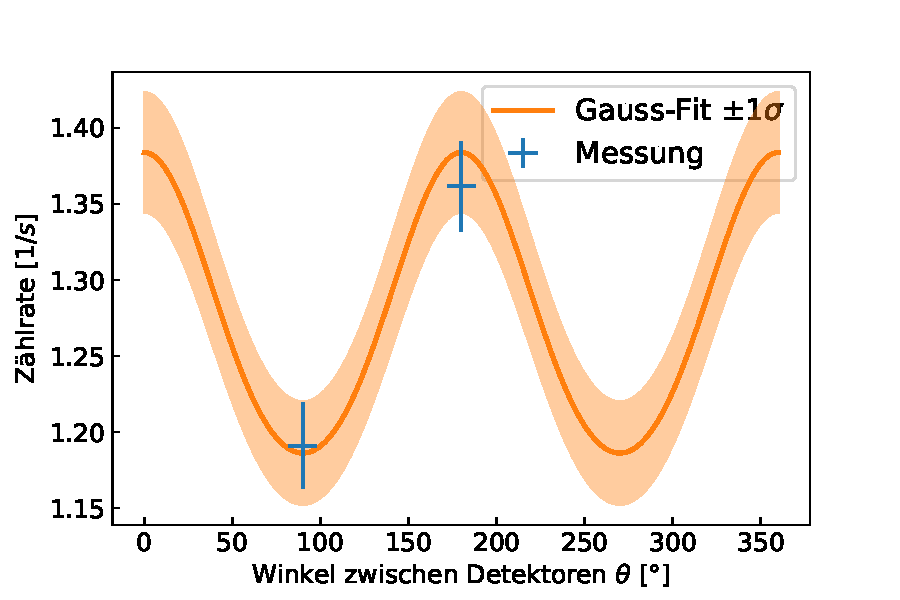
\includegraphics[width=0.7\textwidth]{dat/theoKurve.pdf}
		\caption{Theoretischer Kurvenverlauf und gemessene Einzelwerte.}
		\label{fig:theoKurve}
	\end{figure}
